\documentclass[]{book}
\usepackage{lmodern}
\usepackage{amssymb,amsmath}
\usepackage{ifxetex,ifluatex}
\usepackage{fixltx2e} % provides \textsubscript
\ifnum 0\ifxetex 1\fi\ifluatex 1\fi=0 % if pdftex
  \usepackage[T1]{fontenc}
  \usepackage[utf8]{inputenc}
\else % if luatex or xelatex
  \ifxetex
    \usepackage{mathspec}
  \else
    \usepackage{fontspec}
  \fi
  \defaultfontfeatures{Ligatures=TeX,Scale=MatchLowercase}
\fi
% use upquote if available, for straight quotes in verbatim environments
\IfFileExists{upquote.sty}{\usepackage{upquote}}{}
% use microtype if available
\IfFileExists{microtype.sty}{%
\usepackage{microtype}
\UseMicrotypeSet[protrusion]{basicmath} % disable protrusion for tt fonts
}{}
\usepackage[margin=1in]{geometry}
\usepackage{hyperref}
\hypersetup{unicode=true,
            pdftitle={Rapport de l'OT sur les mobilités résidentielles},
            pdfauthor={Par l'Observatoire des Territoires},
            pdfborder={0 0 0},
            breaklinks=true}
\urlstyle{same}  % don't use monospace font for urls
\usepackage{natbib}
\bibliographystyle{apalike}
\usepackage{longtable,booktabs}
\usepackage{graphicx,grffile}
\makeatletter
\def\maxwidth{\ifdim\Gin@nat@width>\linewidth\linewidth\else\Gin@nat@width\fi}
\def\maxheight{\ifdim\Gin@nat@height>\textheight\textheight\else\Gin@nat@height\fi}
\makeatother
% Scale images if necessary, so that they will not overflow the page
% margins by default, and it is still possible to overwrite the defaults
% using explicit options in \includegraphics[width, height, ...]{}
\setkeys{Gin}{width=\maxwidth,height=\maxheight,keepaspectratio}
\IfFileExists{parskip.sty}{%
\usepackage{parskip}
}{% else
\setlength{\parindent}{0pt}
\setlength{\parskip}{6pt plus 2pt minus 1pt}
}
\setlength{\emergencystretch}{3em}  % prevent overfull lines
\providecommand{\tightlist}{%
  \setlength{\itemsep}{0pt}\setlength{\parskip}{0pt}}
\setcounter{secnumdepth}{5}
% Redefines (sub)paragraphs to behave more like sections
\ifx\paragraph\undefined\else
\let\oldparagraph\paragraph
\renewcommand{\paragraph}[1]{\oldparagraph{#1}\mbox{}}
\fi
\ifx\subparagraph\undefined\else
\let\oldsubparagraph\subparagraph
\renewcommand{\subparagraph}[1]{\oldsubparagraph{#1}\mbox{}}
\fi

%%% Use protect on footnotes to avoid problems with footnotes in titles
\let\rmarkdownfootnote\footnote%
\def\footnote{\protect\rmarkdownfootnote}

%%% Change title format to be more compact
\usepackage{titling}

% Create subtitle command for use in maketitle
\newcommand{\subtitle}[1]{
  \posttitle{
    \begin{center}\large#1\end{center}
    }
}

\setlength{\droptitle}{-2em}

  \title{Rapport de l'OT sur les mobilités résidentielles}
    \pretitle{\vspace{\droptitle}\centering\huge}
  \posttitle{\par}
    \author{Par l'Observatoire des Territoires}
    \preauthor{\centering\large\emph}
  \postauthor{\par}
      \predate{\centering\large\emph}
  \postdate{\par}
    \date{2018-08-02}

\usepackage{booktabs}

\begin{document}
\maketitle

{
\setcounter{tocdepth}{1}
\tableofcontents
}
\chapter{Présentation}\label{presentation}

Voici un \emph{prototype} de ce que pourrait être le rapport de
\textbf{l'observatoire des territoires} qui porte sur les mobilités
résidentielles en France et leur rôle dans l'évolution des territoires.

Il sera publié en 2018. Ou en 2019.

En attendant retrouvez ici les autres publications de l'OT :

\begin{itemize}
\item
  les
  \href{http://www.observatoire-des-territoires.gouv.fr/observatoire-des-territoires/fr/rapports/}{rapports}.
\item
  les
  \href{http://www.observatoire-des-territoires.gouv.fr/observatoire-des-territoires/fr/fiches-danalyse/}{fiches}
\end{itemize}

\begin{figure}
\centering

\includegraphics[width=0.30000\textwidth]{./img/logo_OT.png}
\caption{}
\end{figure}

\chapter{Introduction}\label{intro}

Chaque année, un peu plus de 11\% des personnes résidant en France
déménagent pour un autre logement. Sur 100 personnes mobiles, 35
changent de logement au sein de la même commune, 36 changent de commune
mais restent dans le même département, 11 changent de département au
sein de la même région, et 18 changent de région . Les mobilités
résidentielles sont ainsi à l'origine d'un redéploiement de la
population qui modifie les équilibres territoriaux.

La compréhension de ces dynamiques migratoires et de leurs effets
spatiaux est ainsi au cœur des enjeux actuels et futurs de l'aménagement
des territoires. Dans ce rapport, c'est à une échelle supra-communale
que ces enjeux seront envisagés : bien que l'étude des trajectoires
résidentielles locales soit utile pour adapter la composition du parc de
logements aux besoins, ce document prend plutôt le parti d'une analyse
de plus large échelle (passage d'une agglomération à sa périphérie,
d'une aire urbaine à une autre, d'un département ou d'une région à
l'autre, etc.), qui permet de mesurer les différences d'attractivité des
territoires, et en retour l'effet des mobilités résidentielles sur la
différenciation de ces derniers.

Car s'il existe d'un côté des espaces attractifs, souvent depuis
plusieurs décennies, où croissance migratoire et dynamisme économique
s'entraînent mutuellement , existent aussi de l'autre des zones en
décroissance où le déficit migratoire est autant une conséquence qu'un
facteur aggravant de difficultés souvent liées à la
désindustrialisation. Or, les mobilités résidentielles internes au pays
sont un jeu à somme nulle : un ménage qui s'installe quelque part, c'est
aussi un ménage qui a quitté un autre territoire. \textbf{Les mobilités
résidentielles sont donc au cœur des enjeux de la cohésion
territoriale.}

Certes, l'attractivité migratoire n'est pas le seul ressort du dynamisme
démographique local : les évolutions naturelles de la population
(naissances, décès), très contrastées selon les espaces, y contribuent
aussi largement. En fait, c'est la combinaison -- variable selon les
territoires -- de ces deux dynamiques, migratoire et naturelle, qui
explique les évolutions locales de la population . Néanmoins, une
analyse spécifique du phénomène migratoire est intéressante pour au
moins deux raisons. D'une part, la géographie des mobilités
résidentielles a été en grande partie reconfigurée au cours des
cinquante dernières années, quand celle du solde naturel est au
contraire caractérisée par sa stabilité : les évolutions des mobilités
expliquent donc largement les trajectoires récentes des espaces. D'autre
part, l'attractivité étant depuis peu devenue une préoccupation
grandissante des collectivités territoriales, il est utile d'en montrer
le cadre et les effets à l'échelle nationale : qui sont les Français qui
déménagent, où vont-ils, et quelles conséquences ont ces mobilités sur
la cohésion des territoires : conduisent-elles à les homogénéiser, ou au
contraire à accentuer les disparités ?

\chapter{Déterminants individuels et tendances de la mobilité
résidentielle}\label{determinants-individuels-et-tendances-de-la-mobilite-residentielle}

Le rapport des individus à l'espace et leur propension à changer de
territoire varient selon les étapes du cycle de vie, selon certaines
caractéristiques individuelles, mais aussi selon des facteurs extérieurs
tels que la conjoncture économique et le type de territoire de
résidence. La première partie de ce rapport expose les grandes lignes
des facteurs explicatifs individuels de la mobilité résidentielle de
plus ou moins longue distance, et met ce phénomène en perspective avec
les tendances des dernières décennies et avec les niveaux de mobilité
observés dans les autres pays européens. Les différences de mobilité
selon les types de territoire font quant à elles l'objet de la seconde
partie du rapport.

\section{Une majorité de mobilités résidentielles de
proximité}\label{une-majorite-de-mobilites-residentielles-de-proximite}

bla

\section{De fortes différences de mobilité selon le profil des
individus}\label{de-fortes-differences-de-mobilite-selon-le-profil-des-individus}

bla bla un exemple d'intégration de visuel charté CGET :

\begin{figure}
\centering
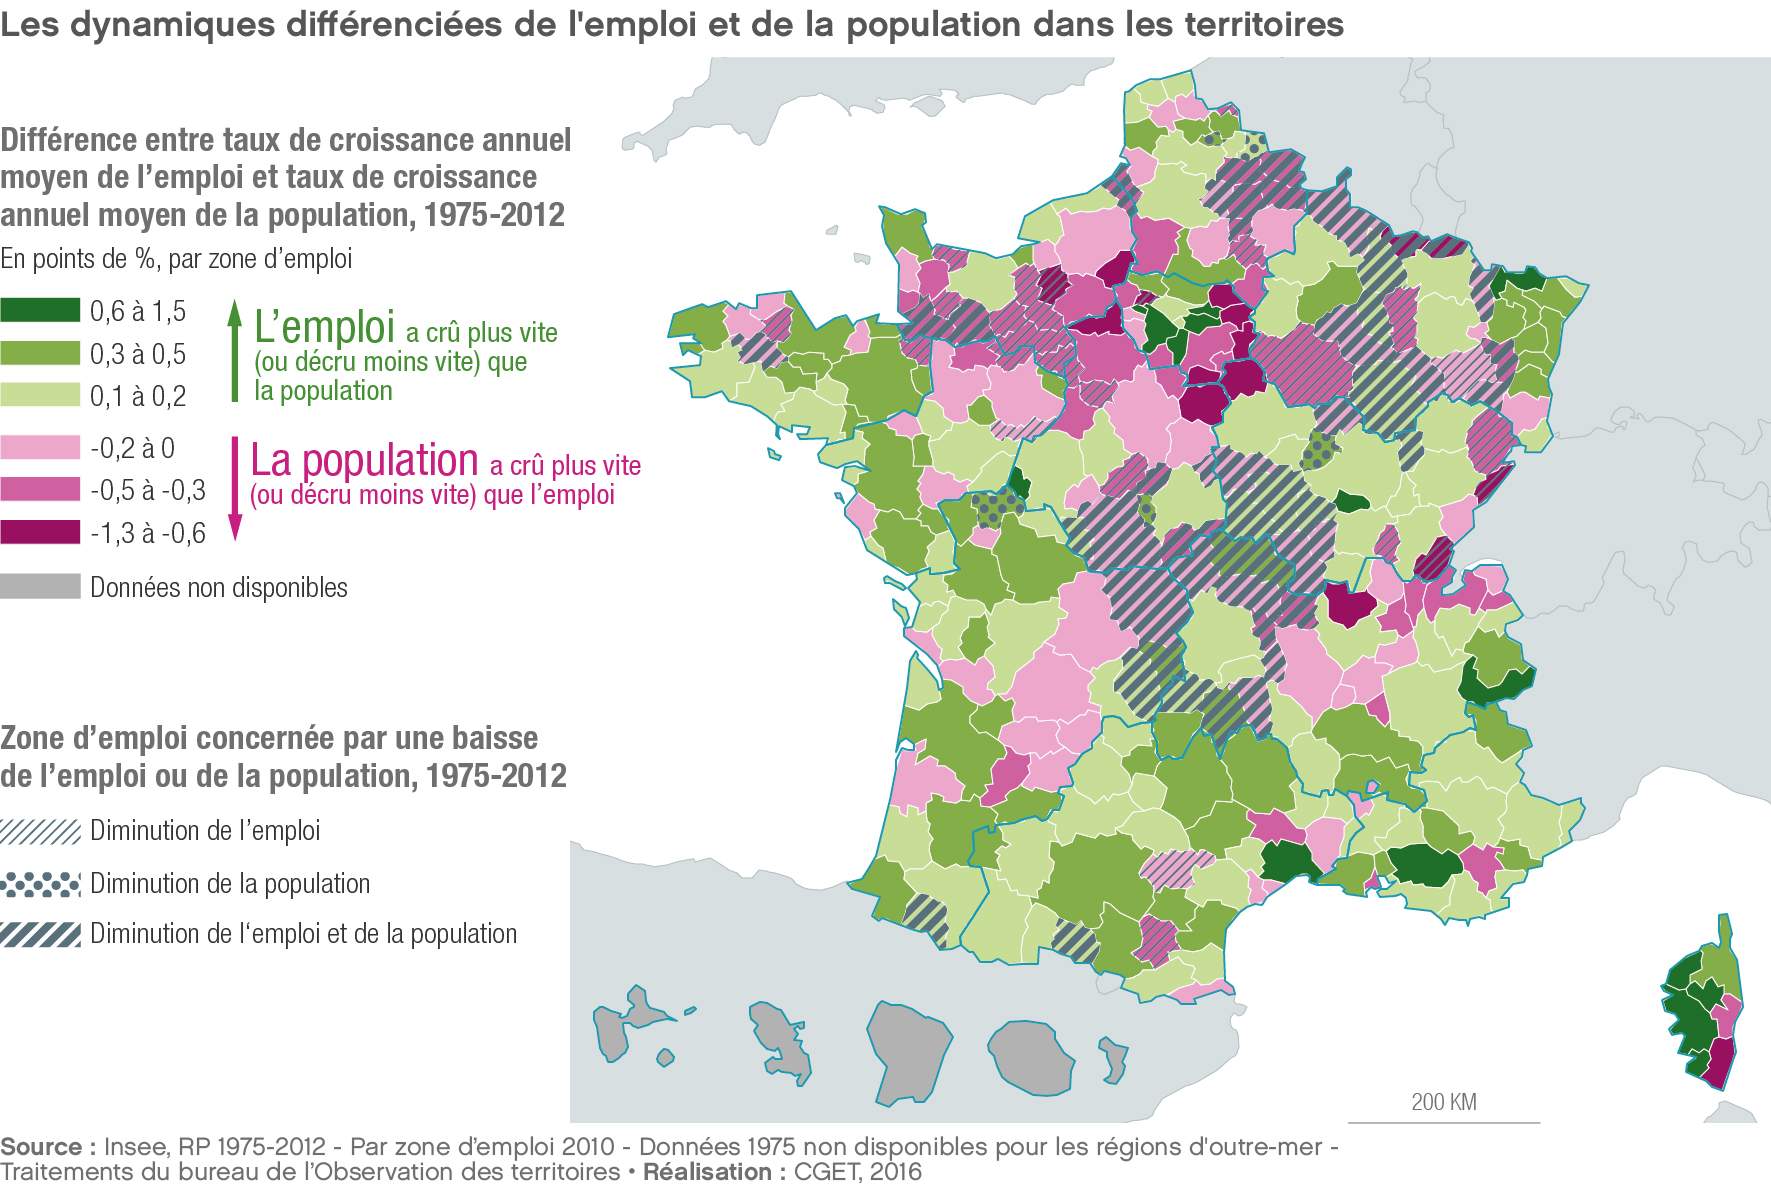
\includegraphics[width=0.80000\textwidth]{./img/1A_Carte5_Diff_Tx_croissance_emploi_pop-01.jpg}
\caption{}
\end{figure}

ou de gif joué depuis R

\url{....}

Des citations à retrouver dans la biblio \textbf{bookdown} package
\citep{R-bookdown} in this sample book, which was built on top of R
Markdown and \textbf{knitr} \citep{xie2015}.

\chapter{Espaces excédentaires et
déficitaires}\label{espaces-excedentaires-et-deficitaires}

\section{Cinquante ans de mobilités : une géographie de l'attractivité
reconfigurée}\label{cinquante-ans-de-mobilites-une-geographie-de-lattractivite-reconfiguree}

Au cours des cinquante dernières années, la géographie des territoires
qui attirent et de ceux que l'on quitte a été profondément renouvelée.
Des espaces qui perdaient de la population sont devenus attractifs,
comme les zones rétro-littorales de l'Ouest et les zones peu denses du
Sud-Ouest, aujourd'hui en pleine expansion. Au contraire, certains
territoires qui étaient attractifs perdent désormais plus d'habitants
qu'ils n'en gagnent au jeu des mobilités résidentielles :
l'Île-de-France et la Côte d'Azur en sont des exemples caractéristiques.

Mais il y a aussi des constantes : une grande partie du Nord-Est connaît
un déficit migratoire depuis plusieurs décennies et l'évolution de la
population n'y est souvent soutenue que par le dynamisme démographique
naturel. Ce chapitre dresse la géographie des mobilités résidentielles
d'aujourd'hui en les inscrivant dans cinquante ans d'évolutions passées,
mais aussi les mettant en perspective avec l'autre ressort de la
croissance démographique : le solde naturel. Une approche « grand angle
» qui a pour vertu de rappeler que les trajectoires des territoires ne
sont pas immuables, ni uniquement tributaires de leur attractivité.

\subsection{Périurbanisation et littoralisation : quand les mobilités
résidentielles construisent le contraste Nord-Est /
Sud-Ouest}\label{periurbanisation-et-littoralisation-quand-les-mobilites-residentielles-construisent-le-contraste-nord-est-sud-ouest}

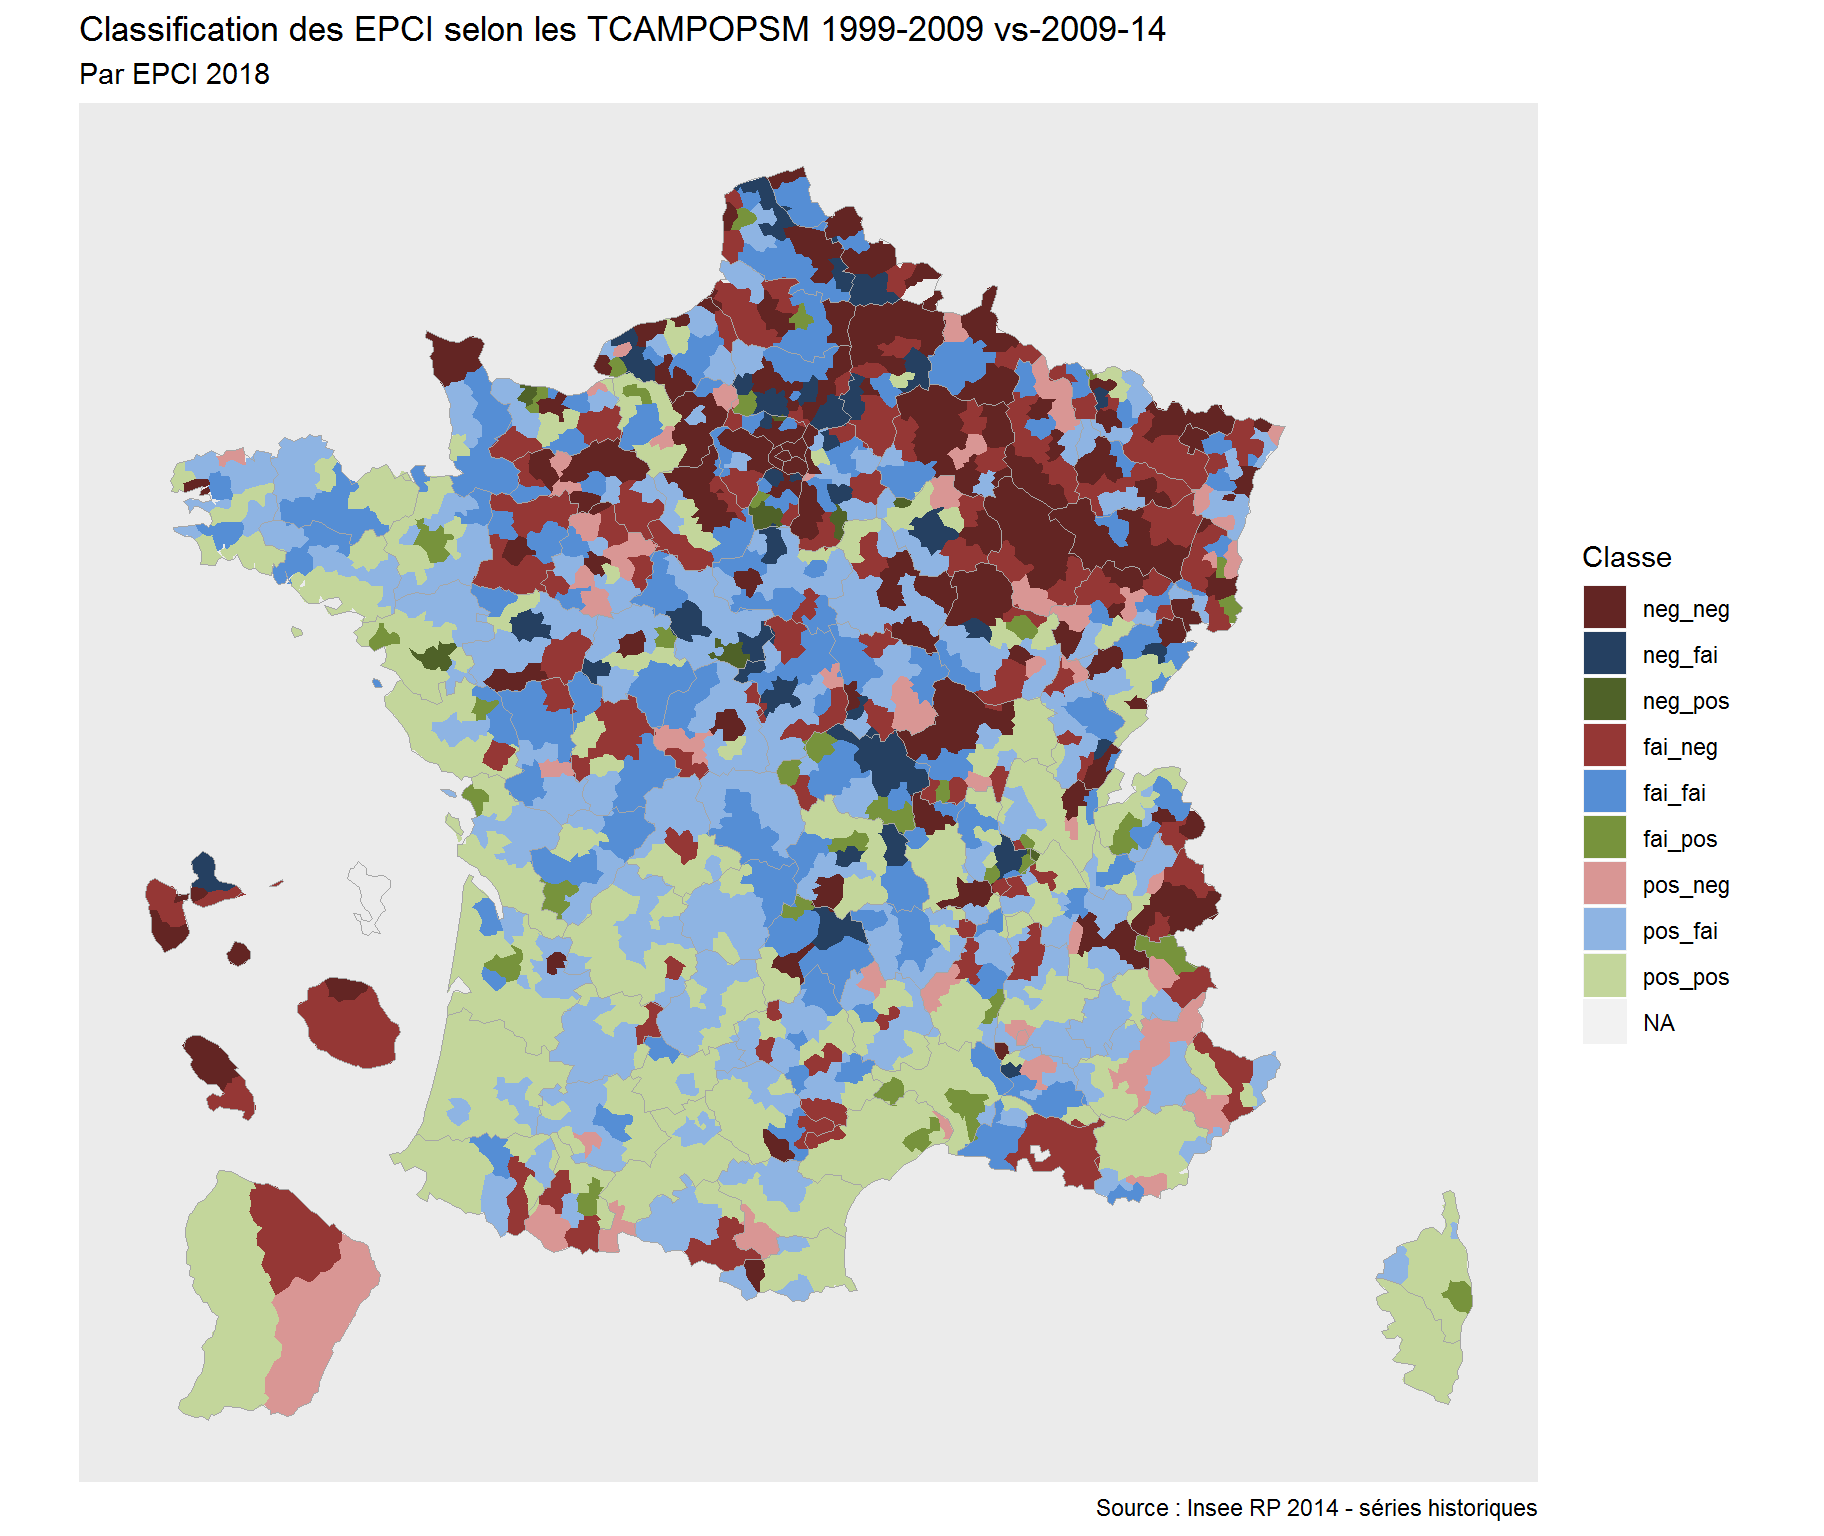
\includegraphics{rapport_OT_mobilites_files/figure-latex/carto_typo_SM_EPCI-1.pdf}

Mais. Mais. Ca bouge !

\includegraphics{rapport_OT_mobilites_files/figure-latex/carto_typo_SM_DEP-1.pdf}

\chapter{Synthèse}\label{synthese}

C'était vraiment très intéressant.


\end{document}
